\section{Transient Absorption}
\label{sec:TRAS}


\begin{table}[ht]
    \centering
    \begin{tabular}{clc}
        \toprule
        Sample No. &    Treatment &    $\tau$ / \si{\nano\second} \\
        \midrule
        1 &     ZnTPP in bn 0.8mM &  $953 \pm 3$ \\
        2 &     ZnTPP in bn 0.6mM &  $972 \pm 4$ \\
        3 &     ZnTPP in bn 0.4mM & $1000 \pm 4$ \\
        4 &     ZnTPP in bn 0.2mM & $1008 \pm 8$ \\
        5 & ZnTPP:C70 in bn 1:0.1 &  $834 \pm 3$ \\
        6 & ZnTPP:C70 in bn 1:0.2 &  $753 \pm 3$ \\
        7 & ZnTPP:C70 in bn 1:0.3 &  $697 \pm 3$ \\
        8 &    ZnTPP in tol 0.8mM &  $533 \pm 1$ \\
        12 &     ZnOEP in bn 0.8mM &  $373 \pm 1$\\
        \bottomrule
    \end{tabular}
\end{table}



\subsection*{Variation in Concentration}
For ZnTPP, different concentrations in bn were measured. From the theory, we expect an exponential decay of the concentration of the triplet 
\begin{equation}
    C_T(t) = C_T(0) \exp[-k_0t],
\end{equation}
with the initital concentration $C_T(0)$ and the decay rate $k_0$.
As the transient absorption $\Delta A(\tau)$ is proportional to $C_T$, we can fit an exponential decay to our data. Hereby, an offset was added to the decay function to correct any offset caused by e.g.~measuring methods. Data and fits are shown in fig.~\ref{fig:TRAS-Conc}.

\begin{figure}[h]
    \centering
    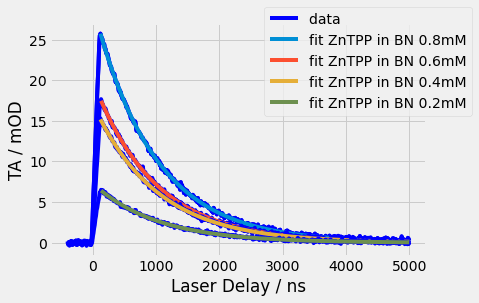
\includegraphics[width = 0.9\textwidth]{Bilder/Auswertung/TRAS/ZnTPPdiffConc.png}
    \caption{Data of the transient absorption of solutions of different concentrations of ZnTPP in bn.}
    \label{fig:TRAS-Conc}
\end{figure}

It is clear, that higher maxima correspond to higher concentrations of ZnTPP. This aligns our expectations as a higher concentration leads to a bigger ammount of absorption. The lifetime $\tau_0$ can be calculated from 
\begin{equation}
    \tau_0 = \frac{1}{k_0}.
\end{equation}

The calculated lifetimes can be found in tab.~\ref{tab:lifetimesConc}.

\begin{table}[ht]
    \centering
    \begin{tabular}{clc}
        \toprule
        Sample No. &    Treatment &    $\tau$ / \si{\nano\second} \\
        \midrule
        1 &     ZnTPP in bn 0.8mM &  $953 \pm 3$ \\
        2 &     ZnTPP in bn 0.6mM &  $972 \pm 4$ \\
        3 &     ZnTPP in bn 0.4mM & $1000 \pm 4$ \\
        4 &     ZnTPP in bn 0.2mM & $1008 \pm 8$ \\
        \bottomrule
    \end{tabular}
    \caption{Calculated lifetimes of ZnTPP solutions in bn with different concentrations.}
    \label{tab:lifetimesConc}
\end{table}

Here, an increasing lifetime for decreasing concentrations of ZnTPP is evident. This aligns our expectations from theory: The kinetics of the decay of the triplet state are determined by the differential equation 
\begin{equation}
    \frac{dC_T(t)}{dt} = - k_1C_T(t) - k_2(C_T(t))^2 - k_3 C_T(t)C_G(t),
\end{equation}
where $C_{T/G}(t)$ is the concentration of the triplet/ground state and $k_{1/2/3}$ are decay rates. In general the assumption is made, that $C_T(t) \ll C_G(t)$, which eventually leads to the exponential decay. However, the decay rate is therefore always underestimated as one process is neglected. Furthermore, the assumption becomes less valid, with an increasing population of the triplet state. Thus, we expect higher decay rates (i.e.~shorter lifetimes) for an increasing concentration of triplet states, which we assigned above to the higher concentrations of ZnTPP. In this way, the decreasing lifetimes for increasing concentrations of ZnTPP can be explained.

\subsection*{Quenching with C\textsubscript{70}}
The lifetime of a triplett state can be reduced by allowing further decay paths. In this experiment, this was achieved by adding different concentrations of the fullerene C\textsubscript{70} to the ZnTPP solutions of \SI{0.8}{\milli\nauticalmile} concentration (solvent:bn). The data and corresponding fits can be seen in fig.~\ref{fig:ZnTPP-C70}. The reduced population of the triplet state for an increasing concentration of fullerene can be seen as an decrease of the maximum transient absorption. The lifetimes can be calculated as shown above. They and the corresponding decay rates are displayed in tab.~\ref{tab:ZnTPP-C70}. As expected, the lifetime decreases with an increasing ammount of fullerene due to more quanching processes being able. 

\begin{figure}[h]
    \centering
    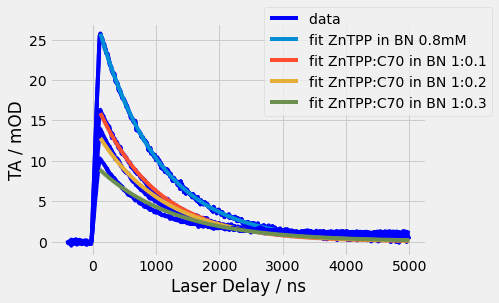
\includegraphics[width = 0.9\textwidth]{Bilder/Auswertung/TRAS/ZnTPP-C70.png}
    \caption{Data of the transient absorption of different dillutions of C\textsubscript{70} in \SI{0.8}{\milli\nauticalmile} ZnTPP in bn.}
    \label{fig:ZnTPP-C70}
\end{figure}

\begin{table}[ht]
    \centering
    \begin{tabular}{clcc}
        \toprule
        Sample No. &    Treatment & $k_{app}$ / \si{\per\milli\second}  &  $\tau$ / \si{\nano\second} \\
        \midrule
        1 &     ZnTPP in bn 0.8mM & $1050 \pm 3$ &  $953 \pm 3$ \\
        5 & ZnTPP:C70 in bn 1:0.1 & $1198 \pm 4$ &  $834 \pm 3$ \\
        6 & ZnTPP:C70 in bn 1:0.2 & $1329 \pm 5$ &  $753 \pm 3$ \\
        7 & ZnTPP:C70 in bn 1:0.3 & $1436 \pm 6$ &  $697 \pm 3$ \\
        \bottomrule
    \end{tabular}
    \caption{Calculated lifetimes of different dillutions of fullerene C\textsubscript{70} in a \SI{0.8}{\milli\nauticalmile} solution in bn.}
    \label{tab:ZnTPP-C70}
\end{table}

To determine the rate of the quenching process $k_q$, the decay rates of the different dillutions $k_{app}$ are plotted against the concentrations of fullerene $[C_{70}]$. Since $k_{app}$ was defined as 
\begin{equation}
    k_{app} = k_0 + k_q C_q,
\end{equation}
$k_q$ corresponds to the slope of the line, which is fitted in fig.~\ref{fig:C70-kq}. A quenching rate of \par 
\centerline{\boxed{k_q =  \SI{1.61 \pm 0.08}{\per\micro\second\per\milli\nauticalmile}}} \par 
was determined. This value does not completely align with the values found by Ito et al., who determined $k_q = $\SI{4.7}{\per\micro\second\per\milli\nauticalmile}~\cite{Nojiri.1998}. Though, the error is within one order of magnitude. 

\begin{figure}[h]
    \centering
    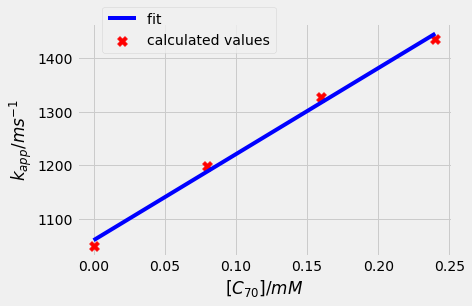
\includegraphics[width = 0.9\textwidth]{Bilder/Auswertung/TRAS/ZnTPP-C70-kq.png}
    \caption{Data of the transient absorption of different dillutions of C\textsubscript{70} in \SI{0.8}{\milli\nauticalmile} ZnTPP in bn.}
    \label{fig:C70-kq}
\end{figure}

%#kyliewarhier

\subsection*{Change of solvent}

In the case of \SI{0.8}{\milli\nauticalmile} ZnTPP, solutions with two different solvents were measured (bn and tol). Analagous to the recent evaluation, the the transient absorption is shown in fig.~\ref{fig:ZnTPP-bn-tol} and the lifetimes were calculated via an exponential decay fit (see tab.~\ref{fig:ZnTPP-bn-tol}).

\begin{figure}[h]
    \centering
    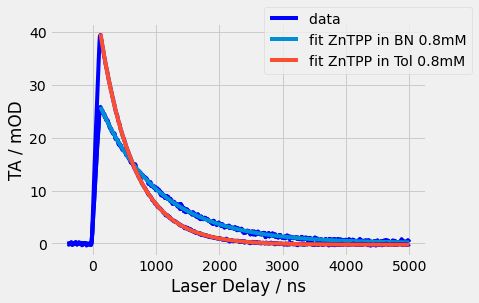
\includegraphics[width = 0.9\textwidth]{Bilder/Auswertung/TRAS/ZnTPP-bn-tol.png}
    \caption{Data of the transient absorption of \SI{0.8}{\milli\nauticalmile} ZnTPP in bn and in tol. For tol a higher maximum transient absorption value was measured.}
    \label{fig:ZnTPP-bn-tol}
\end{figure}


\begin{table}[ht]
    \centering
    \begin{tabular}{clc}
        \toprule
        Sample No. &    Treatment &    $\tau$ / \si{\nano\second} \\
        \midrule
        1 &     ZnTPP in bn 0.8mM &  $953 \pm 3$ \\
        8 &    ZnTPP in tol 0.8mM &  $533 \pm 1$ \\
        \bottomrule
    \end{tabular}
    \caption{Calculated lifetimes of \SI{0.8}{\milli\nauticalmile} ZnTPP solutions in bn and tol.}
    \label{tab:ZnTPP-bn-tol}
\end{table}

It is clear, that ZnTPP in tol shows a higher maximum transient absorption value and a lower lifetime compared to ZnTPP in bn. This aligns with the conclusions of the UV-VIS spectroscopy in~\ref{sec:SSS}. Due to the polarity of bn, charges can be induced more easily in the delocalized $\pi$-electron system. Therefore not only a redshift can be observed. It is further possible, that the stronger resonance stability leads to the increase of lifetime.

\subsection*{Using different zinc complexes}
Not only the zinc complex ZnTPP was measured, but also ZnOEP. Analagous to the recent evaluation, the the transient absorption of \SI{0.8}{\milli\nauticalmile} in bn is shown in fig.~\ref{fig:ZnTPP-ZnOEP} and the lifetimes were calculated via an exponential decay fit (see tab.~\ref{fig:ZnTPP-ZnOEP}).

\begin{figure}[h]
    \centering
    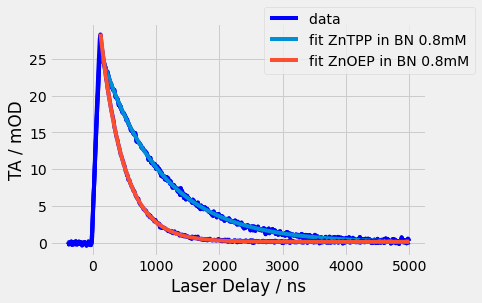
\includegraphics[width = 0.9\textwidth]{Bilder/Auswertung/TRAS/ZnTPP-ZnOEP.png}
    \caption{Data of the transient absorption of \SI{0.8}{\milli\nauticalmile} ZnTPP and ZnOEP in bn. Both complexes have a similar transient absorption value, but ZnOEP shows a faster decay.}
    \label{fig:ZnTPP-ZnOEP}
\end{figure}


\begin{table}[ht]
    \centering
    \begin{tabular}{clc}
        \toprule
        Sample No. &    Treatment &    $\tau$ / \si{\nano\second} \\
        \midrule
        1 &     ZnTPP in bn 0.8mM &  $953 \pm 3$ \\
        12 &     ZnOEP in bn 0.8mM &  $373 \pm 1$\\
        \bottomrule
    \end{tabular}
    \caption{Calculated lifetimes of \SI{0.8}{\milli\nauticalmile} ZnTPP and ZnOEP solutions in bn.}
    \label{tab:ZnTPP-ZnOEP}
\end{table}

While the maximum transient absorption value does not differ much, the lifetime ZnOEP is much shorter than the one for ZnTPP. The maximum TA value corresponds to the maximum concentration of the triplet state and therefore is a measure for the absorption of the pump laser light. The pump laser emits a wavelength of $\lambda = $ \SI{520}{\nano\metre}, which is equivalent to a photon energy of $E_{\gamma} = $ \SI{2.38}{\eV}. When looking at fig.~\ref{fig:ZnTPPZnOEP}, it is clear, that the absorbance at \SI{2.38}{\eV} does not differ much between ZnTPP and ZnOEP. This expains the similar maximum TA values. \par 
The longer lifetime of ZnTPP may again be explained by the redshift compared to ZnOEP, which can be seen in fig.~\ref{fig:ZnTPPZnOEP}. Due to the four additional phenyl groups in ZnTPP, the conjugated electron system is bigger than in ZnOEP a lower energy is needed to exite the electrons of ZnTPP. Also, the resonance stability increases, which might lead to the longer lifetimes measured.

\subsection*{Influence of the pump laser pulse width}
To investigate the influence of the pump laser pulse width on the TA signal, we measured the TA of sample 1 using four different pump laser pulse widths. The resulting plot is illustrated in fig.~\ref{fig:pulsewidth}. It is clear, that the increase is the same for all pulse widths. There is a slight shift in the laser delay time for the begin of the decrease, which is not surprising, since that point marks the end of the laser pulse. The plots only differ in the maximum TA value. This aligns our expectations as a longer pump laser puls width should be able to exite more electrons to the triplet state. To check a possible influence of the pump laser pulse width on the lifetimes $\tau$, those were calculated aswell. As can be seen in tab.~\ref{tab:pulsewidth}, the lifetimes do differ a bit, but there is no overall trend visible. Furthermore, the errors are quite big, probably due to the short measurement time. In respect to the errors we find the values to be the same and therefore see no influence of the pump laser pulse width on the lifetime.

\begin{figure}[h]
    \centering
    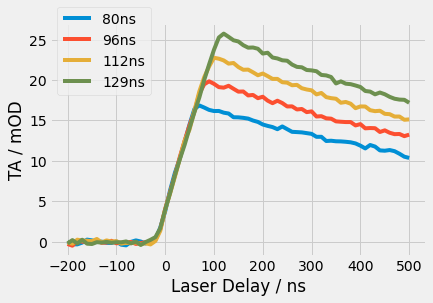
\includegraphics[width = 0.9\textwidth]{Bilder/Auswertung/TRAS/pulsewidth.png}
    \caption{Data of the transient absorption of \SI{0.8}{\milli\nauticalmile} ZnTPP in bn using different pump laser pulse widths. The increase of TA is overall the same. The measurements only differ in the maximum TA value, which is higher for longer pulse widths.}
    \label{fig:pulsewidth}
\end{figure}

\begin{table}[ht]
    \centering
    \begin{tabular}{clc}
        \toprule
        pump laser pulse width / ns & $\tau$ / \si{\micro\second} \\
        \midrule
        80  &     $1 \pm 0.2$ \\
        96  &     $0.9 \pm 0.2$\\
        112 &     $1.1 \pm 0.2$ \\
        129 &     $0.9 \pm 0.1$\\
        \bottomrule
    \end{tabular}
    \caption{Calculated lifetimes of \SI{0.8}{\milli\nauticalmile} ZnTPP in bn for different pump laser pulse widths.}
    \label{tab:pulsewidth}
\end{table}